\section{Vorstellung des Prototypen}\label{prototyp}
Der Prototyp stellt die Bereitstellung von Software an einen Fahrzeughalter dar. Mit der Installierten Software kann das Fahrzeug mit einem Service Provider interagieren. Der Service Provider ist im Kontext des Prototypen ein Parkautomat, über welchen ein Parkticket gebucht werden kann und das Fahrzeug automatisch in eine ihm zugewiesene Parklücke fährt. \\
Da für die Interaktion eine Software notwendig ist, muss diese installiert werden können. Der Prototyp umfasst eine Installation von Software, welche über die Interaktion mit einem Server möglich ist. Kaufentscheidungen bezüglich einer Software aber auch Entscheidungen über die Nutzung eines Service können über eine Android-Schnittstelle (MMS) getätigt werden. Im folgenden werden diese vier Module vorgestellt. Im Anschluss daran werden einzelne weiter erläutert, um so zum Beispiel die Integration von Uptane darzustellen.

\subsection{Architektur des Prototypen}	
Abbildung \hyperref[img:basic]{13} zeigt die Grundlegende Architektur des Prototypen. Die Module "Software Applikation Manager \textit{(\textbf{SAM})}", "Carla Simulation\textit{(\textbf{Carla})"} und die "Mensch-Maschine-Schnittstelle \textit{(\textbf{MMS})"} erstellen zusammen die Repräsentation eines Fahrzeugs, wobei SAM das Herzstück dessen ist. Dieser steuert und organisiert die installierten Softwares eines Fahrzeugs und stellt auch den Kommunikationsmittelpunkt dar. Die Kommunikation mit dem Server zum Kauf einer Software wird über SAM getätigt. Sämtliche Kommunikation als auch sämtliche Entscheidungstreffungen des Fahrzeugs werden hier gesteuert. 
\begin{figure}[!h]
	\centering
	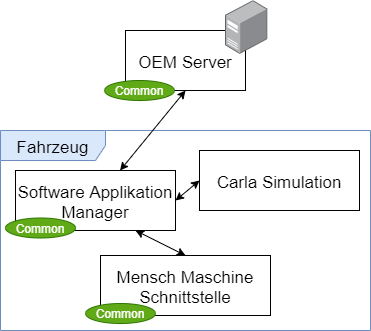
\includegraphics[width=0.5\columnwidth]{pictures/konzept-basic.png}
	\label{img:basic}
	\caption{Grundlegende Architektur der Prototypen}
\end{figure}
Carla stellt die visuelle Repräsentation des Fahrzeug dar. Diese enthält keine Logik, ist im Kontext einer \textit{Model-View-Controller (MVC)}\footnote{MVC Quelle} Architektur demnach als View zu sehen. Die MMS ist sowohl eine visuelle Repräsentation aber auch eine Steuernde Einheit des Prototypen. Zum einen werden über Popups Nachrichten angezeigt, zum anderen kann mittels dieser Popups der Installation einer Software bzw. der Nutzung eines Services zugestimmt werden. Diese Popups werden von einer Software Shop Applikation erstellt.\\
Der "OEM Server \textit{(Server)}" stellt das Backend des Shops dar. Er verwaltet die Software und stellt sie den Fahrzeugen bereit. Sowohl der OEM-S, SAM als auch die MMS sind in Java geschrieben worden. Sie Nutzen zur Kommunikation eine gemeinsame Library aus \textit{Common}-Objekten. Abbildung \hyperref[img:common]{14} zeigt deine generelle Aufteilung in zwei Gruppen, den \textit{Messages} und dem \textit{Environment}. Die Messages sind die Objekte, die zwischen den einzelnen Java-Modulen verschickt. Sie enthalten primitive Werte wie eine ID(int), einen Namen(String) und eine Nachricht(String). Jede Message wird von einer abstrakten "Message"-Klasse abgeleitet. Außerdem hat jede Message eine bestimmte Funktion. Für Details, sehen Sie in das beigelegte Javadoc.
\begin{figure}[!h]
	\centering
	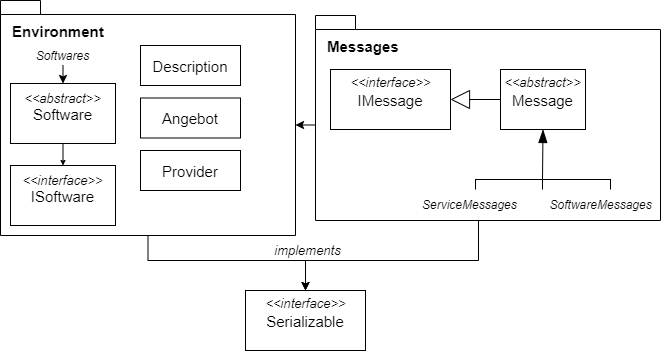
\includegraphics[width=0.8\columnwidth]{pictures/konzept-Common.png}
	\label{img:common}
	\caption{Aufbau der Common Library}
\end{figure}

Außer Primitiven Datentypen können Messages auch "Environment"-Objekte beinhalten. Alle Objekte haben einen bestimmten Zweck. Jede Software, die zum Prototypen hinzugefügt werden soll, muss von der abstrakten Klasse "Software" abgeleitet sein. Diese Abstraktionsebene bietet die Möglichkeit, neue Softwares schnell zum Prototypen hinzufügen zu können. Die einzigen Anforderungen sind ein Konstruktor und eine implementierung der \textit{handleMessage()-}Methode. Neben Software gibt es noch die Description und den Provider. Beide Objekte können jeweils einen Service- als auch einem Software Provider definieren und den Service bzw. die Software beschreiben. Das Angebot repräsentiert die Auswahlmöglichkeiten, die dem Fahrzeughalter beim Kauf einer Software über die MMS vorgeschlagen werden.
\subsubsection{Architektur der Software Applikation Managers (SAM)}
Das Herzstück des Prototypen steuert, was in den anderen Modulen passiert. Wie in Abbildung \hyperref[img:sam]{15} zu sehen, ist SAM in drei einzelne Systeme aufgebaut. In der "Software Control Unit" baut ein Messagehandler eine Kommunikation zwischen SAM, dem Server, aber auch der MMS und Carla auf. Der Messagehandler wertet eingehende Nachrichten aus und passt anhand von ihnen den Ablauf des Prototypen an. Der Messagehandler beinhaltet einen SoftwareManager. Dieser hat die Aufgabe, die Installation neuer Softwares und die Nutzung bereits installierter Softwares zu ermöglichen. Im Messagehandler ankommende Nachrichten beinhalten die ID der Software, welche zum Anzeigen der eingegangenen Nachricht notwendig ist. Der SAM ist mit allen anderen Modulen des Prototypen verbunden. Der Messagehandler baut mit Hilfe der einzelnen Hilfs-Klassen die Verbindung zu allen auf. Die Verbindung mit dem Server wurde über Netty implementiert, die Verbindungen mit der Simulation und der Mensch-Maschine-Schnittstelle wurden durch Sockets und Ports aufgebaut. Hierdurch kann mit dem MessageHandler jedem anderen Modul eine Nachricht gesendet werden.\\

\begin{figure}[!h]
	\centering
	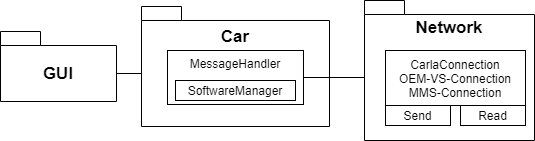
\includegraphics[width=0.5\columnwidth]{pictures/konzept-SAM.png}
	\label{img:sam}
	\caption{Architektur des Software Applikation Managers}
\end{figure}

Um Sämtliche Ereignisse des Prototypen einsehen zu können, wird eine GUI zur Verfügung gestellt. In dieser GUI werden Ereignisse, die in den einzelnen Modulen stattfinden, in diversen Logs aufgelistet. Außerdem kann der Prototyp durch die Nutzung von Knöpfen gesteuert werden. Die Logs sollen im wesentlichen als Gedankenstütze wirken um die Geschehnisse im Ablauf eines Softwareverkaufs aufzulisten.
\subsubsection{Architektur des OEM-Servers (Server)}
\subsection{Installation}
\begin{itemize}
	\item MMS installieren
	\item Carla optional
	\item ccu ausführen
\end{itemize}
\subsection{Funktionen und Nutzung des Prototypen}
\subsubsection{Starten der Einzelsysteme}
richtige Reihenfolge, erklären wieso die beachtet werden sollte. Ob mms oder carla zuerst is irrelevant\\\\
\textbf{Carla}\\
Carla starten\\
cmd aus extrahierten zip-ordner heraus\\
Skript starten: py -3.7 skript\_name.py\\\\
\textbf{MMS}\\

\textbf{SAM\\}
\begin{itemize}
	\item Stages der Simulation (Schritt für Schritt durch den Absatzprozess)
	\item Wie ich von Stage zu Stage komme
	\item stages: no registered car, car in perception area, car leaving, car installing sw, car using service
\end{itemize}
%Sind alle Teilsysteme installiert \textit{(Carla-Installation ist optional)} kann der Anwendungsfall gestartet werden. Im ersten Schritt wird dem Auto signalisiert, dass es in der Simulation losfahren kann. Hierzu muss der "Szenario Starten"-Knopf gedrückt werden. 
\subsection{Analyse der Prototypen und Ausblicke der Weiterentwicklung}
- Mehrwerte aufzählen\\
   Software nutzen auf Autos, welche dem Auto Fahrbefehle gibt.
- Vorteile der gewählten Architektur\\
- Nachteile der gewählten Architektur \& Umsetzung.
